\documentclass{article}

\usepackage{geometry}
\usepackage{graphicx}

\usepackage[utf8]{inputenc}
\usepackage{fourier} 
\usepackage{array}
\usepackage{makecell}

\renewcommand\theadalign{bc}
\renewcommand\theadfont{\bfseries}
\renewcommand\theadgape{\Gape[4pt]}
\renewcommand\cellgape{\Gape[4pt]}

\geometry{letterpaper, left=1cm, right=1cm, top=1.5cm, bottom=2cm}

\title{Adversarial Images}
\author{Adam Spindler}

\begin{document}
\maketitle

\section{Introduction}

\section{Accuracies with Perturbation}

\subsection{Adding Noise}
\begin{center}
\begin{tabular}{ c c c c }
    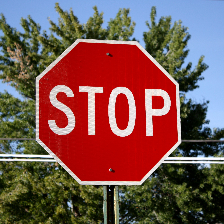
\includegraphics[width=0.2\linewidth]{../test_images/stop.png} & 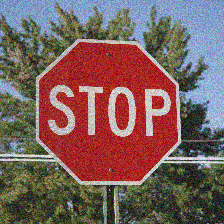
\includegraphics[width=0.2\linewidth]{../test_images/perturbed/stop_noise_100.png} & 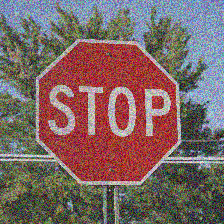
\includegraphics[width=0.2\linewidth]{../test_images/perturbed/stop_noise_200.png} & 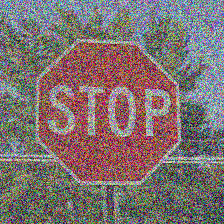
\includegraphics[width=0.2\linewidth]{../test_images/perturbed/stop_noise_500.png} \\
    \makecell{YOLOv3 = 0.99987 \\ RCNN = 0.99987} & \makecell{YOLOv3 = 0.99987 \\ RCNN = 0.99993} & \makecell{YOLOv3 = 0.99968 \\ RCNN = 0.99610} & \makecell{YOLOv3 = 0.99985 \\ RCNN = 0} \\  
    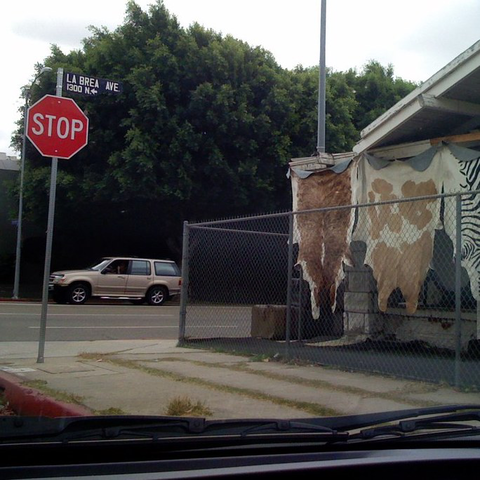
\includegraphics[width=0.2\linewidth]{../test_images/stop3.png} & 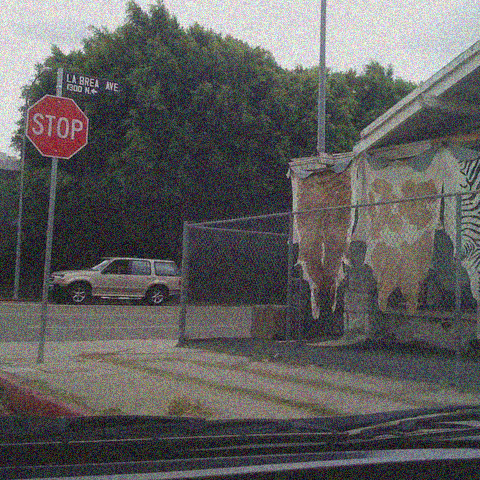
\includegraphics[width=0.2\linewidth]{../test_images/perturbed/stop3_noise_100.png} & 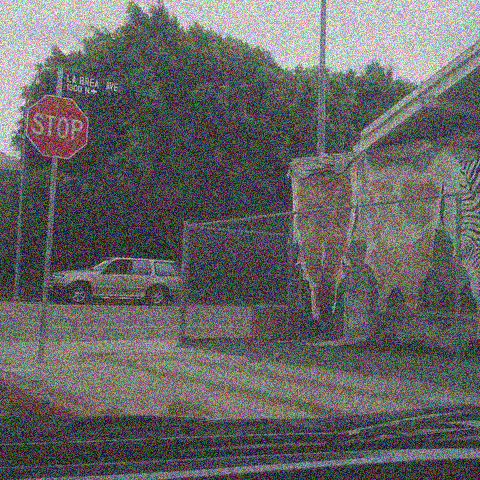
\includegraphics[width=0.2\linewidth]{../test_images/perturbed/stop3_noise_200.png} & 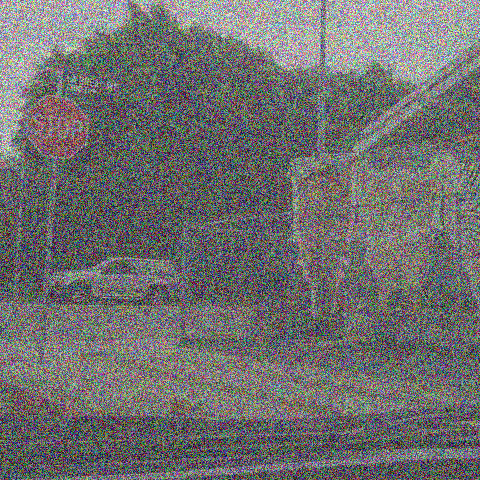
\includegraphics[width=0.2\linewidth]{../test_images/perturbed/stop3_noise_500.png} \\
    \makecell{YOLOv3 = 0.99971 \\ RCNN = 0.99839} & \makecell{YOLOv3 = 0.99995 \\ RCNN = 0.99926} & \makecell{YOLOv3 = 0.99951 \\ RCNN = 0.99850} & \makecell{YOLOv3 = 0 \\ RCNN = 0} \\  
\end{tabular}
\end{center}

\subsection{Grayscale}
\begin{center}
\begin{tabular}{ c c c c }
    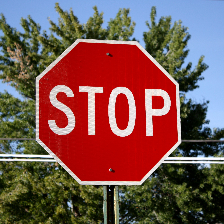
\includegraphics[width=0.2\linewidth]{../test_images/stop.png} & 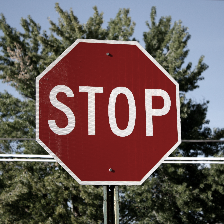
\includegraphics[width=0.2\linewidth]{../test_images/perturbed/stop_grayscale_0_500.png} & 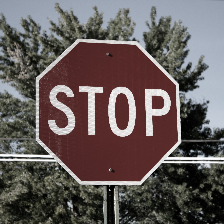
\includegraphics[width=0.2\linewidth]{../test_images/perturbed/stop_grayscale_0_250.png} & 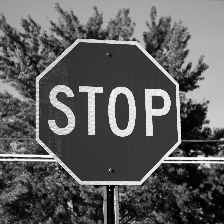
\includegraphics[width=0.2\linewidth]{../test_images/perturbed/stop_grayscale_0_010.png} \\
    \makecell{YOLOv3 = 0.99987 \\ RCNN = 0.99987} & \makecell{YOLOv3 = 0.99988 \\ RCNN = 0.99987} & \makecell{YOLOv3 = 0.99989 \\ RCNN = 0.99986} & \makecell{YOLOv3 = 0.99986 \\ RCNN = 0.99868} \\  
    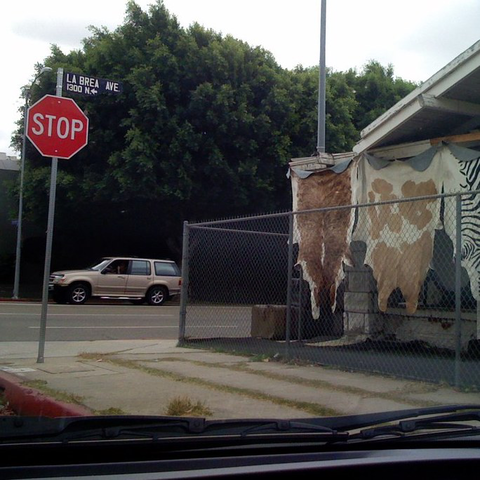
\includegraphics[width=0.2\linewidth]{../test_images/stop3.png} & 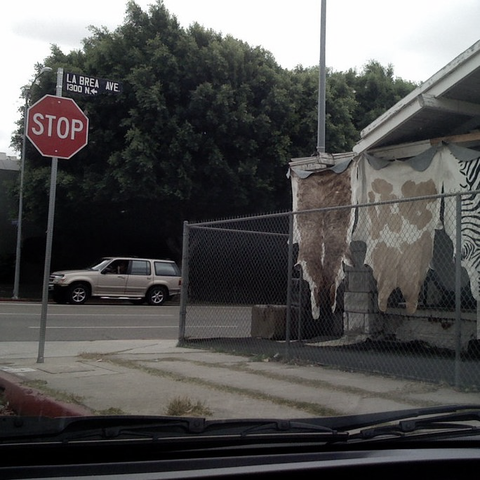
\includegraphics[width=0.2\linewidth]{../test_images/perturbed//stop3_grayscale_0_500.png} & 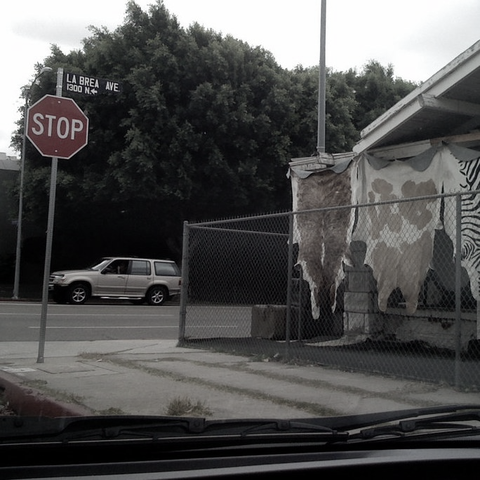
\includegraphics[width=0.2\linewidth]{../test_images/perturbed/stop3_grayscale_0_250.png} & 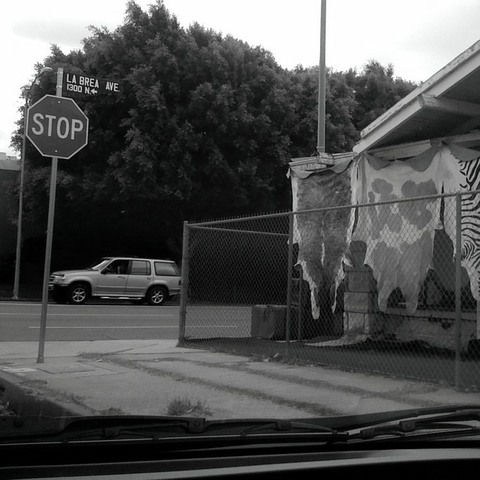
\includegraphics[width=0.2\linewidth]{../test_images/perturbed/stop3_grayscale_0_010.png} \\
    \makecell{YOLOv3 = 0.99971 \\ RCNN = 0.99839} & \makecell{YOLOv3 = 0.99971 \\ RCNN = 0.99859} & \makecell{YOLOv3 = 0.99970 \\ RCNN = 0.99866} & \makecell{YOLOv3 = 0.99965 \\ RCNN = 0.99846} \\  
\end{tabular}
\end{center}

\subsection{Contrast}
\begin{center}
\begin{tabular}{ c c c c }
    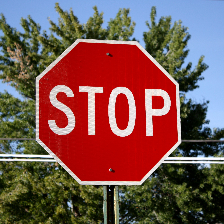
\includegraphics[width=0.2\linewidth]{../test_images/stop.png} & 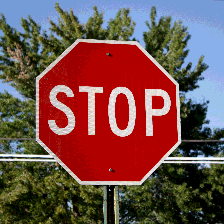
\includegraphics[width=0.2\linewidth]{../test_images/perturbed/stop_contrast_0_050.png} & 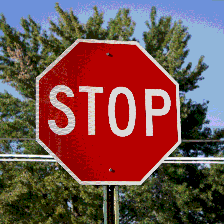
\includegraphics[width=0.2\linewidth]{../test_images/perturbed/stop_contrast_0_025.png} & 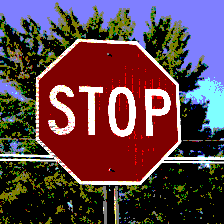
\includegraphics[width=0.2\linewidth]{../test_images/perturbed/stop_contrast_0_010.png} \\
    \makecell{YOLOv3 = 0.99987 \\ RCNN = 0.99987} & \makecell{YOLOv3 = 0.99985 \\ RCNN = 0.99994} & \makecell{YOLOv3 = 0.99986 \\ RCNN = 0.99993} & \makecell{YOLOv3 = 0.99984 \\ RCNN = 0.99859} \\  
    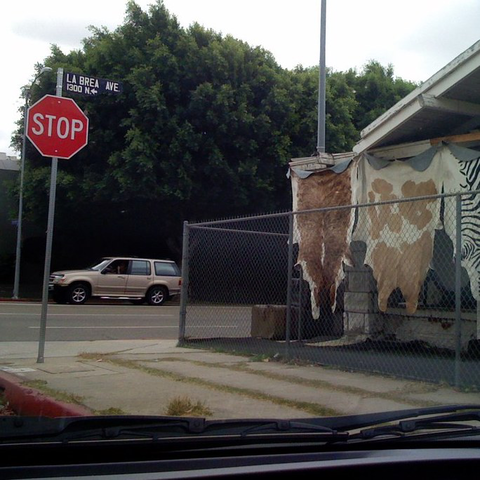
\includegraphics[width=0.2\linewidth]{../test_images/stop3.png} & 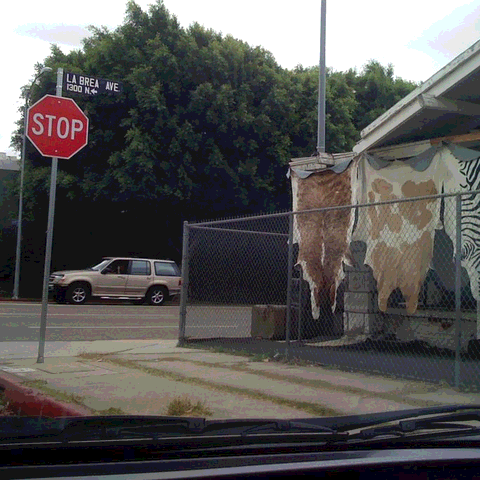
\includegraphics[width=0.2\linewidth]{../test_images/perturbed/stop3_contrast_0_050.png} & 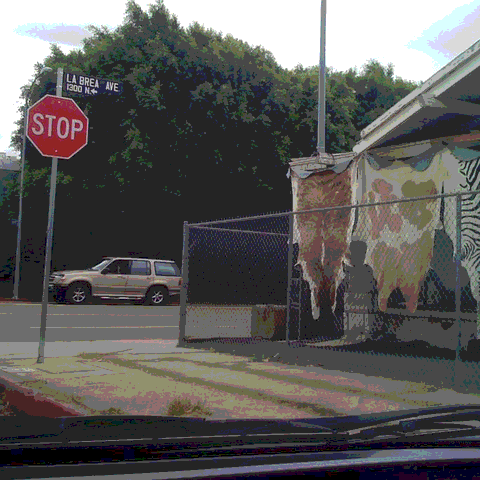
\includegraphics[width=0.2\linewidth]{../test_images/perturbed/stop3_contrast_0_025.png} & 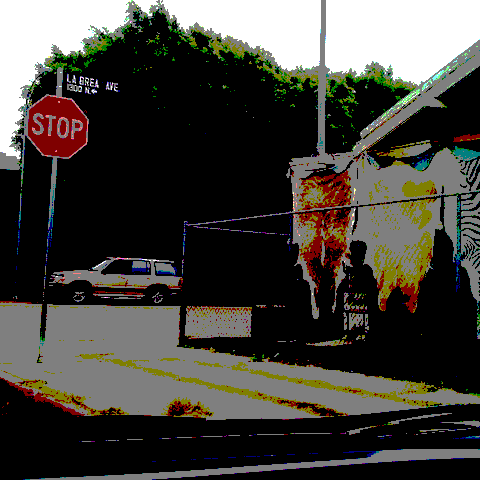
\includegraphics[width=0.2\linewidth]{../test_images/perturbed/stop3_contrast_0_010.png} \\
    \makecell{YOLOv3 = 0.99971 \\ RCNN = 0.99839} & \makecell{YOLOv3 = 0.99961 \\ RCNN = 0.99849} & \makecell{YOLOv3 = 0.99960 \\ RCNN = 0.99830} & \makecell{YOLOv3 = 0.99990 \\ RCNN = 0.99893} \\  
\end{tabular}
\end{center}

\end{document}